\documentclass[12pt]{article}

\usepackage{sbc-template}

\usepackage{graphicx,url}

\usepackage[brazil]{babel}   
%\usepackage[latin1]{inputenc}  

     
\sloppy

\title{Instructions for Authors of SBC Conferences\\ Papers and Abstracts}

\author{Vitor Mendes paisante}


\address{Departamento de Ciência da Computação da Universidade Federal de Minas Gerais
  \email{\{paisante\}@dcc.ufmg.br}
}

\begin{document} 

\maketitle

\begin{abstract}
Alias analysis is one of the most fundamental techniques that
compilers use to optimize languages with pointers.
However, in spite of all the attention that this topic has received, the current
state-of-the-art approaches inside compilers still face challenges regarding
precision and speed.
In particular, pointer arithmetic, a key feature in C and C++, is yet to be
handled satisfactorily.
This work presents a new alias analysis algorithm to solve this problem.
The key insight of our approach is to combine alias analysis with symbolic
range analysis.
This combination lets us disambiguate fields within arrays and structs,
effectively achieving more precision than traditional algorithms.
To validate our technique, we have implemented it on top of the LLVM compiler.
Tests on a vast suite of benchmarks show that we can disambiguate several
kinds of C idioms that current state-of-the-art analyses cannot deal with.
In particular, we can disambiguate 1.35x more queries than the alias analysis
currently available in LLVM.
Furthermore, our analysis is very fast: we can go over one million assembly
instructions in 10 seconds..
\end{abstract}
     

\section {Context}
% the importance of Alias Analysis
Pointer analysis is one of the most fundamental compiler technologies.
This analysis lets the compiler distinguish one memory location from others;
hence, it provides the necessary information to transform code that manipulates
memory.
Given this importance, it comes as no surprise that pointer analysis has been
one of the most researched topics within the field of compiler
construction\cite{Hind01}.
This research has contributed to make the present algorithms more
precise~\cite{Hardekopf07a,Zhang14}, and faster~\cite{Hardekopf11,Shang12}.
Nevertheless, one particular feature of imperative programming languages remains
to be handled satisfactorily by the current state-of-the-art approaches:
the disambiguation of pointer intervals.

\section {Problem}
% The problem imposed by pointer arithmetics and The need for better alias analyses.
Mainstream compilers still struggle to distinguish intervals within the
same array.
In other words, state-of-the-art pointer analyses often fail to disambiguate
regions addressed from a common base pointer via different
offsets, as explained by Yong and Horwitz~\cite{Yong04}. Figure 
\ref{fig:intro_ex} shows an example that state-of-the-art pointer analyses 
tend not to deal with satisfactorily. In the example, both stores on the $r$ 
array posses different offsets and they do not alias. To figure out that such 
offsets are disjoint it is necessary to verify their ranges and add a new layer
of analysis to the current pointer analyses available.

\begin{figure}[t!]
  \centering
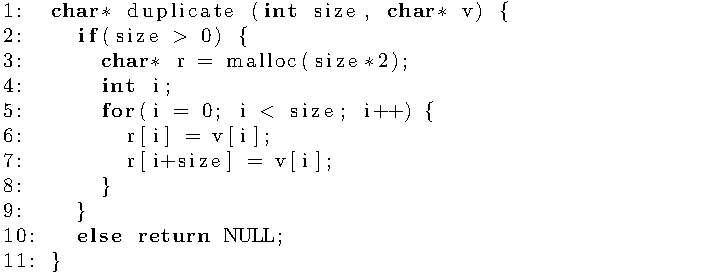
\includegraphics[width=\linewidth]{img/introex}
  \caption{Example that state-of-the-art pointer analyses handle 
  unsatisfactorily.}
  \label{fig:intro_ex}
\end{figure}

Field-sensitive pointer analysis, provide a partial solution to this problem.
These analyses can distinguish different fields within a record, such
as a struct in C~\cite{Pearce04}, or a class in Java~\cite{Yan11}.
However, they rely on syntax that is usually absent in the low level program
representations adopted by compilers.
Shape analyses~\cite{Jones82,Sagiv98} can disambiguate subparts of
data-structures such as arrays, yet their scalability remains an issue to be
solved.
Consequently, many compiler optimizations, such as
loop transformations, tiling, fission, skewing and
interchanging~\cite[Ch.09]{Wolfe96}, are very limited in practice.
Therefore, we claim that, to reach their full potential, compilers need to
be provided with more effective alias analyses.

\section {Solution}
% Combining alias and range analyses.
This work describes such an analysis.
We introduce an abstract domain that associates pointers with symbolic ranges.
In other words, for each pointer $p$ we conservatively estimate the range of
memory slots that can be addressed as an offset of $p$.
We let $>(p)$ be the global abstract address set associated with pointer $p$, 
such that if
$loc{i} + [l, u] \in >(p)$, then $p$ may dereference any address
from $@(loc{i}) + l$ to $@(loc{i}) + u$,
where $loc{i}$ is a program site that
contains a memory allocation call, and $@(loc{i})$ is the actual return
address of the {\em malloc} at runtime.
We let $\{ l, u \}$ be two {\em symbols} defined within the program code.
Like the vast majority of pointer analyses available in the compiler
literature, from Andersen's work~\cite{Andersen94} to the more recent 
technique of Zhang {\em et al.}~\cite{Zhang14}, our method is correct if the
underlying program is also correct.
In other words, our results are sound with respect to the semantics of the
program if this program has no undefined behavior, such as out-of-bounds
accesses.

\textbf{The key insight of our research} is the combination of pointer analysis
with range analysis on the symbolic interval lattice.
In a symbolic range analysis, ranges are defined as expressions of the program's
symbols, a symbol being either a constant or the name of a variable.
There exist many approaches to symbolic range analyses in the
literature~\cite{Blume94,Nazare14,Rugina05}.
The algorithms that we present in this work do not depend on any particular
implementation.
Nevertheless, the more precise the range analysis that we use, the more
precise the analysis facts that we produce.
In this work we have adopted the symbolic range analysis proposed in 1994 by
William Blume and Rudolf Eigenmann~\cite{Blume94}.

\section {Summary of experimental results}
To validate our ideas, we have implemented them in the LLVM compilation
infra-structure~\cite{Lattner04}.
We have tested our pointer analysis onto three different benchmarks
used in previous work related to pointer disambiguation:
Prolangs~\cite{Ryder01}, PtrDist~\cite{Zhao05} and MallocBench~\cite{Grunwald93}.
As we show in Chapter \ref{chap:exp}, our analysis is linear on the size of
programs.
It can go over one-million assembly instructions in approximately 10 seconds.
Furthermore, we can disambiguate 1.35x more queries than the alias analysis
currently available in LLVM.

\section {Summary of publications}
The analysis described here was published on the International Symposium on 
Code Generation and Optimization (CGO) of 2016 held in Barcelona, Spain 
\cite{Paisante16}. 

The technology behind it is also present on two other publications 
\cite{Paisante14, Saggioro15}. In these papers, the algorithm presented here was used
to infer the layout and the content of buffers transfered through the network. 
This was useful for verifying, in a safe communication line, if the information 
transfered between two programs through a network should be considered potentially 
dangerous or not. If proven not dangerous, guards for checking integer overflows
may not be necessary. These articles proposed methods for such verification to 
be used on the internet of things (IoT), where simple devices could run 
significantly faster with a reduced number of integer overflow checks. 
The layout and content inference analysis used in these papers differed from our 
current approach by using a numerical range analysis, since a symbolic approach 
would not be of relevance for such application.

\section {Limitations}
%- Limitations of the current analysis
Using the symbolic range analysis for comparing offsets is inherently 
imprecise. Issues lie on comparing two symbolic expressions and its 
difficulties, especially on comparing lower bounds with upper bounds from two
different variables, and on local relationships of variables with overlapping 
ranges.

Figure \ref{fig:lim1} shows the first issue. Analyzing this algorithm, the 
symbolic range analysis returns the following ranges: $R(\sigma_a) = [a, b-1]$,
$R(\sigma_b) = [a+1, b]$. This hinders the disambiguation of the two array 
accesses, $V[\sigma_a]$ and $V[\sigma_b]$, since it is impossible to prove that
 the ranges of $\sigma_a$ and $\sigma_b$ do not overlap. To do so, it would be 
 necessary for the valuation of symbolic expressions to be able to say that 
 $b-1 < a+1$ or that $b < a$, which it cannot do. So in this example, even 
 though it is obvious that the two array accesses cannot alias to the same 
 location since their offsets are obligatorily different by the \textbf{if} 
 condition, we cannot disambiguate them. 
 
Figure \ref{fig:lim2} shows the second issue. It again shows two array accesses 
that are obviously disjoint that our analysis cannot disambiguate. Analyzing this 
algorithm, the symbolic range analysis returns the following ranges: 
$R(i) = [0, 9]$, $R(j) = [1, 10]$. It's clear that these ranges overlap and 
that our analysis could not say that they are disjoint even though, at the 
array accesses, $j$ is aways different and greater than $i$. 

These examples show two very interesting limitations of our analysis. They 
both can disable optimizations such as automatic parallelization of code and 
loop invariant code motion on some cases in which these optimizations might be 
desirable. It is clear that simply verifying if two offset ranges are disjoint 
is not enough to achieve ideal precision, since they can hide relationships 
between variables that are aways true when the two variables are alive and 
that can help in disambiguating two pointers, even if there is a relationship 
between these pointers or between the offsets that constitute such pointers. 
 

\begin{figure}[t!]
  \centering
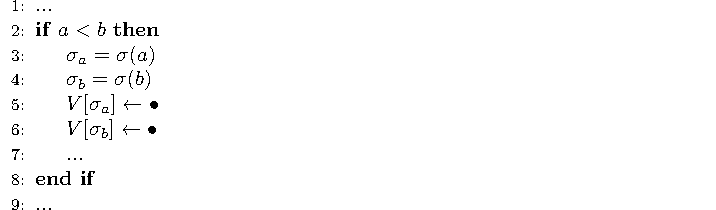
\includegraphics[width=\linewidth]{img/limitation}
  \caption{Example of our first described limitation. Even though we cannot 
  prove that the symbolic ranges of $\sigma_a$ and $\sigma_b$ do not overlap, 
  it is obvious that $\sigma_a$ is aways different from $\sigma_b$ because of 
  the \textbf{if} condition.}
  \label{fig:lim1}
\end{figure}

\begin{figure}[t!]
  \centering
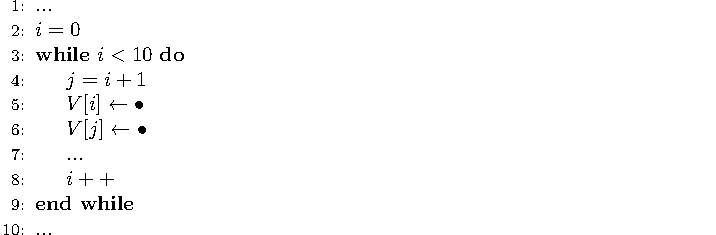
\includegraphics[width=\linewidth]{img/limitation2}
  \caption{Example of our second described limitation. Even though we cannot 
  prove that the ranges of $i$ and $j$ do not overlap, 
  it is obvious that $j$ is aways different from $i$ because it is 
  aways greater.}
  \label{fig:lim2}
\end{figure}

\section {Future Work}
The reason for the limitations exposed before lays on the fact that our analysis 
use range intervals to disambiguate pointers.
In the examples of figure \ref{fig:lim1} and figure \ref{fig:lim2}, the ranges 
of integer variables might either overlap or aren't comparable. But, in the 
examples, variables do have relationships between them that allow for 
disambiguation in the form of inequalities ($a<b$ and $i<j$). To take advantage 
of such relationships we intend to use a lattice similar to Pentagons.

Pentagons is an abstract domain invented by Logozzo and F\"{a}hndrich
to infer symbolic bounds to the integer variables used in
programs \cite{Logozzo08,Logozzo10}.
This abstract domain is formed by the combination of two
lattices.
The first lattice is the {\em integer interval domain} \cite{Cousot77}, which
maps integer variables to ranges $[l, u]$ of numeric lower ($l$) and upper ($u$)
bounds.
The second lattice is the {\em strict upper bound}, which maps each variable
$v$ to a set $L_<$ of other variables, so that if $u \in L_<(v)$, at a given
program point $\mathtt{p}$, then $u < v$ at $\mathtt{p}$. 

Since their debut \cite{Logozzo08}, Pentagons have been used in several
different ways.
For instance, Logozzo and F\"{a}hndrich have employed this domain to eliminate
array bound checks in strongly typed programming
languages \cite{Logozzo10}, and to ensure absence of division by zero or
integer overflows in programs.
Moreover, Nazar\'{e} {\em et al.} \cite{Nazare14} have used Pentagons to reduce
the overhead imposed by AddressSanitizer \cite{Serebryany12} to guard C against
out-of-bounds memory accesses.
The appeal of pentagons comes from two facts.
First, this abstract domain can be computed efficiently -- in quadratic time on
the number of program variables.
Second, as an enabler of compiler optimizations, Pentagons have been
proven to be substantially more effective than other forms of abstract
interpretation of similar runtime \cite{Logozzo08}.

%- Future Work
Our initial and recent use of pentagons for such purpose has been successful. 
It is able to handle programs as large as SPEC's gcc in a few minutes and go
through SPEC CPU 2006 \cite{Henning06} in able time. It has proven very 
useful in some cases, such as SPEC \texttt{470.lbm}.  
In future work, we plan to investigate better splitting strategies
and other more expressive lattices to improve the global precision of
our analyses.

\section {Final Conclusions}
%- Final Conclusions
In this work we have presented a new alias analysis technique that handles,
within the same theoretical framework, the subtleties of pointer arithmetic
and memory indexation.
Our technique can disambiguate regions within arrays and C-like structs using
the same abstract interpreter.
We have achieved precision in our algorithm by combining
alias analysis with classic range analysis on the symbolic domain.
Our analysis is fast, and handles cases that the implementations of
pointer analyses currently available in LLVM cannot deal with.

Apart from this contribution, there is plenty to study on the area of 
pointer analysis, and the area of pointer arithmetics still needs quite a bit 
of research. Their dire needs are very efficient static analyses that run fast on 
very big programs, and very lean dynamic analyses. Our focus has 
been on the static analysis side. Lazy implementations, where main computations 
are made on the query moment, seem to be a very promising take on alias 
analyses and can expedite runtime. Focus on integrating new proposals to 
bigger compilation frameworks and existing optimizations should also be explored 
by the community on an effort of making new technology more usable across 
researchers and projects. There is still a lot of work to be done and we hope 
that our contribution can be only a building block of a much bigger effort from 
many more scientists.

\bibliographystyle{sbc}
\bibliography{bibfile}

\end{document}
